\documentclass{beamer}
\usepackage{listings,xcolor,epsf,mathrsfs}
\usepackage{graphicx} % Allows including images
\usepackage{booktabs} % Allows the use of \toprule, \midrule and \bottomrule in tables
%\usetheme{Warsaw}
\usetheme{Madrid}
\newcommand{\pa}{\partial}
\newcommand{\di}{\displaystyle}
\begin{document}
 \mode<presentation>

\title[Mathematical Analysis I]{A Presentation on Mathematical Analysis I}
\author{ Teo Lee Peng}


\date{\today}
\institute[XMUM]{Department of Mathematics\\ Xiamen University Malaysia}

\begin{frame}
\titlepage
\end{frame}




\begin{frame}
\frametitle{Introduction }
\framesubtitle{\it{This project is about continuity.}}

\vspace{0.5cm}
\begin{itemize}

\item This is a template about presentation slides using latex beamer.

\item A hyperbolic surface of finite type is a surface of genus $g$, with $q$ punctures, and $v$ elliptic points. Its fundamental group is generated by $2g$ hyperbolic elements, $q$ parabolic elements and $v$ elliptic elements of finite orders $m_1$, $m_2$, $\ldots$, $m_v$. Such a surface is called a surface of type $(g;q;m_1, m_2, \ldots, m_v)$ with
    $$2g-2+q+\sum_{j=1}^v\left(1-\frac{1}{m_j}\right)>0$$
\end{itemize}

\end{frame}

\begin{frame}
\frametitle{Classification of M$\ddot{\text{o}}$bius Transformations  }
\begin{itemize}

\item Given $\di \gamma=\begin{pmatrix} a & b\\c&d\end{pmatrix}\in \text{PSL}\,(2,\mathbb{R})$,
its fixed point   satisfies $az+b=(cz+d)z$. Namely,
$$z=\frac{a-d\pm\sqrt{(a-d)^2-4bc}}{2c}=\frac{a-d\pm\sqrt{(a+d)^2-4 }}{2c}$$

\vspace{0.3cm}
\item $\gamma$ is

\vspace{0.3cm}
\begin{itemize}
\item Elliptic if $|a+d|<2$.

\vspace{0.3cm}
\item Parabolic if $|a+d|=2$.

\vspace{0.3cm}
\item Hyperbolic if $|a+d|>2$.

\end{itemize}


\end{itemize}


\end{frame}

 
\begin{frame}
\frametitle{Figure and Citation }
\begin{itemize}\item  This is an example of figure.

\begin{figure}[h]
  \centering
  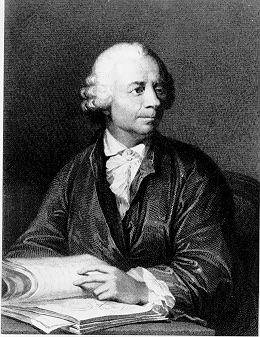
\includegraphics[scale=0.3 ]{euler}
  \caption{A picture of Euler.} \label{c1.F.Euler}
\end{figure}

\item Let us cite the reference book for latex \cite{Latex}. 
\end{itemize}
\end{frame}

\begin{frame}
\frametitle{More Examples of Citations}
Here are some examples on how to cite articles in a collection, journal papers and books. The article \cite{Tao} is in the book \emph{Random Matrices}. 
 The reference \cite{Denton} is a journal paper, and the reference \cite{Oksendal2005} is a book. 
\end{frame}


\begin{frame}
\frametitle{There Is No Largest Prime Number}
\framesubtitle{The proof uses \textit{reductio ad absurdum}.}
\begin{theorem}
There is no largest prime number.
\end{theorem}
\begin{proof}
\begin{enumerate}
\item<1-| alert@1> Suppose $p$ were the largest prime number.
\item<2-> Let $q$ be the product of the first $p$ numbers.
\item<3-> Then $q+1$ is not divisible by any of them.
\item<1-> Thus $q+1$ is also prime and greater than $p$.\qedhere
\end{enumerate}
\end{proof}
\end{frame}

 

\begin{frame}\frametitle{}


\hspace{4cm}{\Huge  Thank You}



\end{frame}

\begin{frame}\frametitle{References}
  
%\bibliography{refs}   %refs.bib is the bibliography database
%\bibliographystyle{alpha} % alphabetical style

 \begin{thebibliography}{}

\bibitem[DPTZ22]{Denton}
Peter Denton, Stephen Parke, Terence Tao, and Xining Zhang.
\newblock Eigenvectors from eigenvalues: {A} survey of a basic identity in
  linear algebra.
\newblock {\em Bull. Amer. Math. Soc. (N.S.)}, 59(1):31--58, 2022.

\bibitem[GH16]{Latex}
David~F. Griffiths and Desmond~J. Higham.
\newblock {\em Learning {L}a{T}e{X}}.
\newblock Society for Industrial and Applied Mathematics (SIAM), Philadelphia,
  PA, second edition, 2016.

\bibitem[{\O}ks05]{Oksendal2005}
B~{\O}ksendal.
\newblock {\em Stochastic differential equations: an introduction with
  application}.
\newblock Springer-Verlag, Berlin, 6th edition, 2005.
\end{thebibliography}
\end{frame}

\begin{frame}\frametitle{References}
  
%\bibliography{refs}   %refs.bib is the bibliography database
%\bibliographystyle{alpha} % alphabetical style

 \begin{thebibliography}{}
\bibitem[Tao19]{Tao}
Terence Tao.
\newblock Least singular value, circular law, and {L}indeberg exchange.
\newblock In {\em Random matrices}, volume~26 of {\em IAS/Park City Math.
  Ser.}, pages 461--498. Amer. Math. Soc., Providence, RI, 2019.

\end{thebibliography}

\vfill
 \end{frame}
\end{document} 